\documentclass{standalone}
\usepackage{tikz}
\usetikzlibrary{patterns, positioning}


\begin{document}
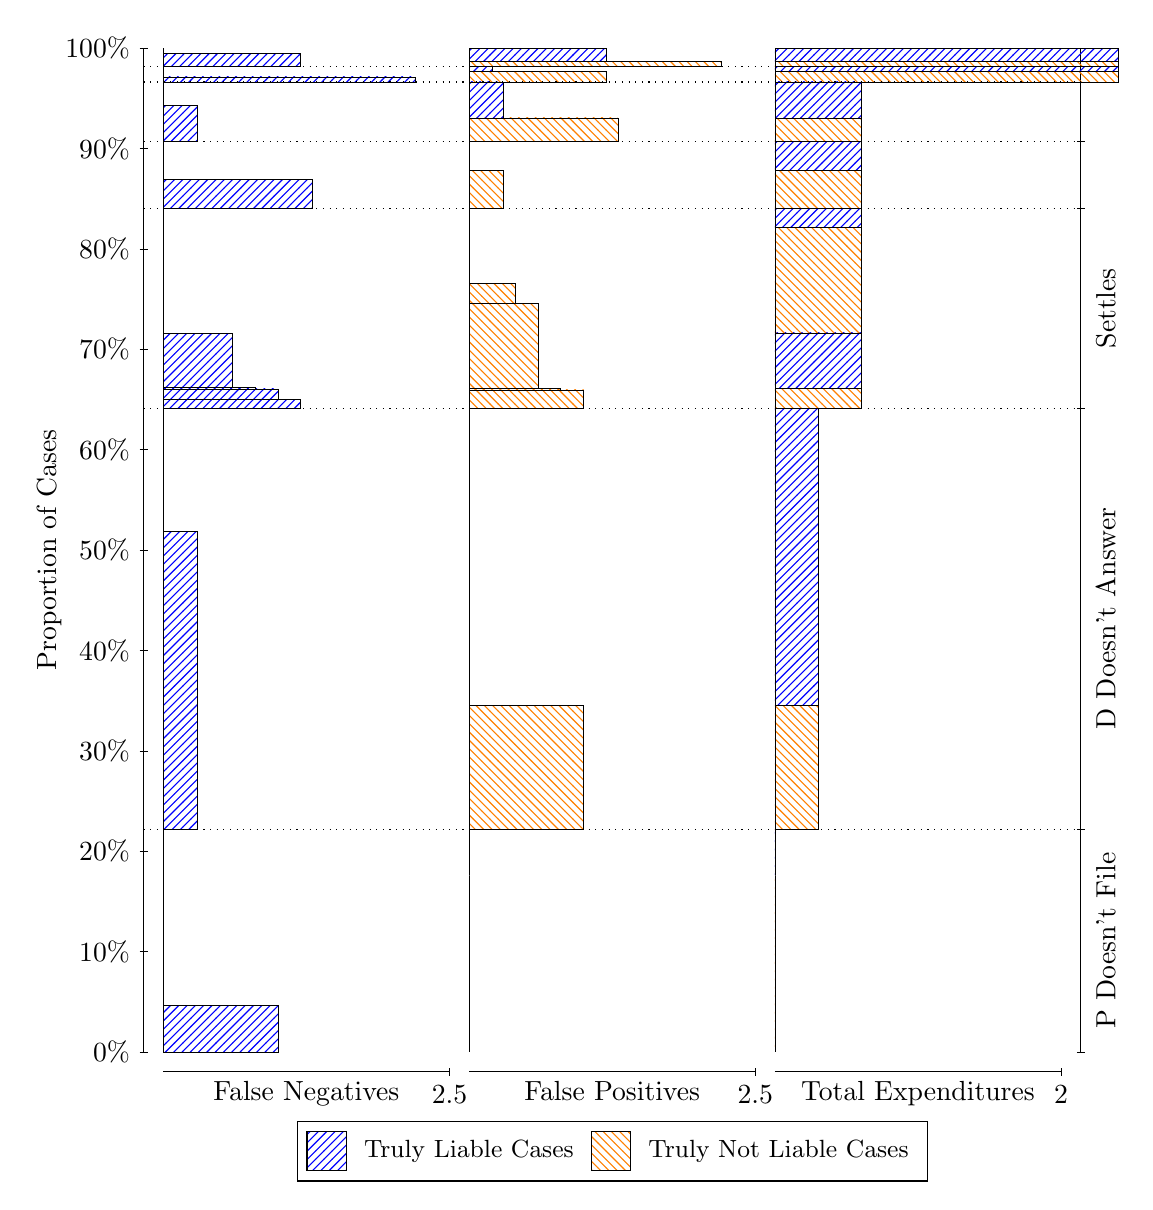
\begin{tikzpicture}
\draw[black, very thin] (1.5,1.75) -- (1.5,14.5);
\node[rotate=90, text=black, anchor=center] at (0.3, 8.125) {Proportion of Cases};
\draw[black, very thin] (1.45,1.75) -- (1.55,1.75);
\node[text=black, anchor=east] at (1.45, 1.75) {0\%};
\draw[black, very thin] (1.45,3.025) -- (1.55,3.025);
\node[text=black, anchor=east] at (1.45, 3.025) {10\%};
\draw[black, very thin] (1.45,4.3) -- (1.55,4.3);
\node[text=black, anchor=east] at (1.45, 4.3) {20\%};
\draw[black, very thin] (1.45,5.575) -- (1.55,5.575);
\node[text=black, anchor=east] at (1.45, 5.575) {30\%};
\draw[black, very thin] (1.45,6.85) -- (1.55,6.85);
\node[text=black, anchor=east] at (1.45, 6.85) {40\%};
\draw[black, very thin] (1.45,8.125) -- (1.55,8.125);
\node[text=black, anchor=east] at (1.45, 8.125) {50\%};
\draw[black, very thin] (1.45,9.4) -- (1.55,9.4);
\node[text=black, anchor=east] at (1.45, 9.4) {60\%};
\draw[black, very thin] (1.45,10.675) -- (1.55,10.675);
\node[text=black, anchor=east] at (1.45, 10.675) {70\%};
\draw[black, very thin] (1.45,11.95) -- (1.55,11.95);
\node[text=black, anchor=east] at (1.45, 11.95) {80\%};
\draw[black, very thin] (1.45,13.225) -- (1.55,13.225);
\node[text=black, anchor=east] at (1.45, 13.225) {90\%};
\draw[black, very thin] (1.45,14.5) -- (1.55,14.5);
\node[text=black, anchor=east] at (1.45, 14.5) {100\%};

\draw[black, very thin] (13.4,1.75) -- (13.4,14.5);
\draw[black, very thin] (13.35,1.75) -- (13.45,1.75);
\node[anchor=west] at (13.35, 1.75) {};
\draw[black, very thin] (13.35,4.5811) -- (13.45,4.5811);
\node[anchor=west] at (13.35, 4.5811) {};
\draw[black, very thin] (13.35,9.9275) -- (13.45,9.9275);
\node[anchor=west] at (13.35, 9.9275) {};
\draw[black, very thin] (13.35,12.464) -- (13.45,12.464);
\node[anchor=west] at (13.35, 12.464) {};
\draw[black, very thin] (13.35,13.315) -- (13.45,13.315);
\node[anchor=west] at (13.35, 13.315) {};
\draw[black, very thin] (13.35,14.069) -- (13.45,14.069);
\node[anchor=west] at (13.35, 14.069) {};
\draw[black, very thin] (13.35,14.269) -- (13.45,14.269);
\node[anchor=west] at (13.35, 14.269) {};
\draw[black, very thin] (13.35,14.5) -- (13.45,14.5);
\node[anchor=west] at (13.35, 14.5) {};

\draw[black, very thin, pattern color=blue, pattern=north east lines] (1.75,1.75) rectangle (3.2033,2.3374);
\draw[black, very thin, pattern color=orange, pattern=north west lines] (1.75,2.3374) rectangle (1.75,4.5811);
\draw[black, very thin, pattern color=blue, pattern=north east lines] (1.75,4.5811) rectangle (2.186,8.3598);
\draw[black, very thin, pattern color=orange, pattern=north west lines] (1.75,8.3598) rectangle (1.75,9.9275);
\draw[black, very thin, pattern color=blue, pattern=north east lines] (1.75,9.9275) rectangle (3.494,10.033);
\draw[black, very thin, pattern color=blue, pattern=north east lines] (1.75,10.033) rectangle (3.2033,10.171);
\draw[black, very thin, pattern color=blue, pattern=north east lines] (1.75,10.171) rectangle (2.9127,10.187);
\draw[black, very thin, pattern color=blue, pattern=north east lines] (1.75,10.187) rectangle (2.622,10.878);
\draw[black, very thin, pattern color=orange, pattern=north west lines] (1.75,10.878) rectangle (1.75,12.464);
\draw[black, very thin, pattern color=blue, pattern=north east lines] (1.75,12.464) rectangle (3.6393,12.833);
\draw[black, very thin, pattern color=orange, pattern=north west lines] (1.75,12.833) rectangle (1.75,13.315);
\draw[black, very thin, pattern color=blue, pattern=north east lines] (1.75,13.315) rectangle (2.186,13.772);
\draw[black, very thin, pattern color=orange, pattern=north west lines] (1.75,13.772) rectangle (1.75,14.069);
\draw[black, very thin, pattern color=blue, pattern=north east lines] (1.75,14.069) rectangle (4.9473,14.133);
\draw[black, very thin, pattern color=orange, pattern=north west lines] (1.75,14.133) rectangle (1.75,14.269);
\draw[black, very thin, pattern color=blue, pattern=north east lines] (1.75,14.269) rectangle (3.494,14.436);
\draw[black, very thin, pattern color=orange, pattern=north west lines] (1.75,14.436) rectangle (1.75,14.5);
\draw[black, very thin, pattern color=orange, pattern=north west lines] (5.6333,1.75) rectangle (5.6333,3.9937);
\draw[black, very thin, pattern color=blue, pattern=north east lines] (5.6333,3.9937) rectangle (5.6333,4.5811);
\draw[black, very thin, pattern color=orange, pattern=north west lines] (5.6333,4.5811) rectangle (7.0867,6.1488);
\draw[black, very thin, pattern color=blue, pattern=north east lines] (5.6333,6.1488) rectangle (5.6333,9.9275);
\draw[black, very thin, pattern color=orange, pattern=north west lines] (5.6333,9.9275) rectangle (7.0867,10.159);
\draw[black, very thin, pattern color=orange, pattern=north west lines] (5.6333,10.159) rectangle (6.796,10.175);
\draw[black, very thin, pattern color=orange, pattern=north west lines] (5.6333,10.175) rectangle (6.5053,11.261);
\draw[black, very thin, pattern color=orange, pattern=north west lines] (5.6333,11.261) rectangle (6.2147,11.513);
\draw[black, very thin, pattern color=blue, pattern=north east lines] (5.6333,11.513) rectangle (5.6333,12.464);
\draw[black, very thin, pattern color=orange, pattern=north west lines] (5.6333,12.464) rectangle (6.0693,12.945);
\draw[black, very thin, pattern color=blue, pattern=north east lines] (5.6333,12.945) rectangle (5.6333,13.315);
\draw[black, very thin, pattern color=orange, pattern=north west lines] (5.6333,13.315) rectangle (7.5227,13.612);
\draw[black, very thin, pattern color=blue, pattern=north east lines] (5.6333,13.612) rectangle (6.0693,14.069);
\draw[black, very thin, pattern color=orange, pattern=north west lines] (5.6333,14.069) rectangle (7.3773,14.205);
\draw[black, very thin, pattern color=blue, pattern=north east lines] (5.6333,14.205) rectangle (5.924,14.269);
\draw[black, very thin, pattern color=orange, pattern=north west lines] (5.6333,14.269) rectangle (8.8307,14.333);
\draw[black, very thin, pattern color=blue, pattern=north east lines] (5.6333,14.333) rectangle (7.3773,14.5);
\draw[black, very thin, pattern color=orange, pattern=north west lines] (9.5167,1.75) rectangle (9.5167,3.9937);
\draw[black, very thin, pattern color=blue, pattern=north east lines] (9.5167,3.9937) rectangle (9.5167,4.5811);
\draw[black, very thin, pattern color=orange, pattern=north west lines] (9.5167,4.5811) rectangle (10.062,6.1488);
\draw[black, very thin, pattern color=blue, pattern=north east lines] (9.5167,6.1488) rectangle (10.062,9.9275);
\draw[black, very thin, pattern color=orange, pattern=north west lines] (9.5167,9.9275) rectangle (10.607,10.175);
\draw[black, very thin, pattern color=blue, pattern=north east lines] (9.5167,10.175) rectangle (10.607,10.883);
\draw[black, very thin, pattern color=orange, pattern=north west lines] (9.5167,10.883) rectangle (10.607,12.22);
\draw[black, very thin, pattern color=blue, pattern=north east lines] (9.5167,12.22) rectangle (10.607,12.464);
\draw[black, very thin, pattern color=orange, pattern=north west lines] (9.5167,12.464) rectangle (10.607,12.945);
\draw[black, very thin, pattern color=blue, pattern=north east lines] (9.5167,12.945) rectangle (10.607,13.315);
\draw[black, very thin, pattern color=orange, pattern=north west lines] (9.5167,13.315) rectangle (10.607,13.612);
\draw[black, very thin, pattern color=blue, pattern=north east lines] (9.5167,13.612) rectangle (10.607,14.069);
\draw[black, very thin, pattern color=orange, pattern=north west lines] (9.5167,14.069) rectangle (13.877,14.205);
\draw[black, very thin, pattern color=blue, pattern=north east lines] (9.5167,14.205) rectangle (13.877,14.269);
\draw[black, very thin, pattern color=orange, pattern=north west lines] (9.5167,14.269) rectangle (13.877,14.333);
\draw[black, very thin, pattern color=blue, pattern=north east lines] (9.5167,14.333) rectangle (13.877,14.5);
\draw[black, dotted] (1.5,4.5811) -- (13.4,4.5811);
\draw[black, dotted] (1.5,9.9275) -- (13.4,9.9275);
\draw[black, dotted] (1.5,12.464) -- (13.4,12.464);
\draw[black, dotted] (1.5,13.315) -- (13.4,13.315);
\draw[black, dotted] (1.5,14.069) -- (13.4,14.069);
\draw[black, dotted] (1.5,14.269) -- (13.4,14.269);
\draw[black, very thin] (1.75,1.5) -- (5.3833,1.5);
\node[text=black, anchor=north] at (3.5667, 1.5) {False Negatives};
\draw[black, very thin] (5.3833,1.45) -- (5.3833,1.55);
\node[text=black, anchor=north] at (5.3833, 1.45) {2.5};

\draw[black, very thin] (5.6333,1.5) -- (9.2667,1.5);
\node[text=black, anchor=north] at (7.45, 1.5) {False Positives};
\draw[black, very thin] (9.2667,1.45) -- (9.2667,1.55);
\node[text=black, anchor=north] at (9.2667, 1.45) {2.5};

\draw[black, very thin] (9.5167,1.5) -- (13.15,1.5);
\node[text=black, anchor=north] at (11.333, 1.5) {Total Expenditures};
\draw[black, very thin] (13.15,1.45) -- (13.15,1.55);
\node[text=black, anchor=north] at (13.15, 1.45) {2};

\node[text=black, centered, rotate=90] at (13.72, 3.1655) {P Doesn't File};
\node[text=black, centered, rotate=90] at (13.72, 7.2543) {D Doesn't Answer};
\node[text=black, centered, rotate=90] at (13.72, 11.196) {Settles};





\draw (7.449999999999999,1.5) node[draw=none] (baseCoordinate) {};
\begin{scope}[align=center]
        \matrix[scale=0.5, draw=black, below=0.5cm of baseCoordinate, nodes={draw}, column sep=0.1cm]{
            \node[rectangle, draw, minimum width=0.5cm, minimum height=0.5cm, pattern color=blue, pattern=north east lines] {}; &
            \node[draw=none, font=\small, text=black] (B) {Truly Liable Cases}; &
            \node[rectangle, draw, minimum width=0.5cm, minimum height=0.5cm, pattern color=orange, pattern=north west lines] {}; &
            \node[draw=none, font=\small, text=black] (B) {Truly Not Liable Cases}; \\
            };
\end{scope}

\end{tikzpicture}
\end{document}